% ===== CHAPTER 11 =====
\chapter{多电子原子}
\label{chap:11}
\section{Hartree-Fock自洽场方法}
\label{sec:11.1 The Hartree-Fock Self-Consistent-Field Method}

    对于氢原子,其精确波函数是已知的。对于氦和锂,通过在变分函数中引入电子间距离,已经计算出了非常精确的波函数。对于原子序数较高的原子,找到精确波函数的一种方法是首先使用Hartree–Fock方法找到一个近似波函数,我们将在本节中概述该方法。Hartree-Fock方法是多电子系统中使用原子和分子轨道的基础。

    $n$电子原子的哈密顿算符为
    \begin{equation}
        \hat{H} = -\frac{\hbar^2}{2m_{\mathrm{e}}} \sum_{i=1}^{n} \nabla_i^2 - \sum_{i=1}^{n} \frac{Z \mathrm{e}^2}{4\pi\varepsilon_0 r_i} + \sum_{i=1}^{n-1} \sum_{j=i+1}^{n} \frac{\mathrm{e}^2}{4\pi\varepsilon_0 r_{ij}}
        \label{eq:11.1}
    \end{equation}
    其中假设存在一个质量无限大的点状原子核(第\ref{sec:6.6 The Bound-State Hydrogen-Atom Wave Functions}节)。(\ref{eq:11.1})中的第一个求和包含了$n$个电子的动能算符。第二个求和为电子和核电荷$Z\mathrm{e}$之间的吸引势(\ref{eq:6.58})。对于中性原子,有$Z=n$。最后一个求和为电子排斥势。限制$j > i$避免了重复计算电子间排斥力,且舍去了如$\mathrm{e}^2/4\pi\varepsilon_0 r_{ii}$这样的项。哈密顿算符(\ref{eq:11.1})是不完整的,因为它忽略了自旋轨道和其他相互作用。略去的项较小(除了具有高$Z$值的原子,它们将在第\ref{sec:11.6 Spin-Orbit Interaction}和\ref{sec:11.7 The Atomic Hamiltonian}节中讨论。

\subsection*{Hartree自洽场方法}

    由于电子间排斥项$\mathrm{e}^2 / 4\pi\varepsilon_0r_{ij}$的存在,单原子的薛定谔方程无法分离变量。回忆处理氦原子的微扰法(第\ref{sec:9.3 Perturbation Treatment of the Helium-Atom Ground State}节),通过忽略这些排斥项,我们可以得到零级波函数。那么薛定谔方程就可以分离成$n$个单电子类氢方程。零级波函数就是$n$个类氢(单电子)轨道的乘积:
    \begin{equation}
        \psi^{(0)} = f_1(r_1, \theta_1, \phi_1) f_2(r_2, \theta_2, \phi_2) \cdots f_n(r_n, \theta_n, \phi_n)
        \label{eq:11.2}
    \end{equation}
    其中类氢轨道为
    \begin{equation}
        f = R_{nl}(r) Y_{l}^m(\theta, \phi)
        \label{eq:11.3}
    \end{equation}
    对于原子的基态,我们将两个自旋相反的电子放入最低能级轨道中,这符合泡利不相容原理,从而得到基态组态。虽然近似波函数 (\ref{eq:11.2}) 在定性上很有用,但在定量精度方面却存在严重缺陷。首先,所有轨道都使用了完整的核电荷数$Z$。回顾我们对氦和锂的变分处理,我们知道可以通过为不同轨道使用不同的有效原子数来考虑电子的屏蔽效应,从而获得更好的近似。使用有效原子数会带来显著的改进,但我们与获得一个准确的波函数仍相去甚远。下一步是使用与(\ref{eq:11.2})形式相同的变分函数,但不限于类氢原子或其他特定轨道形式。因此,我们采用
    \begin{equation}
        \phi = g_1\left(r_1, \theta_1, \phi_1\right) g_2\left(r_2, \theta_2, \phi_2\right) \cdots g_n\left(r_n, \theta_n, \phi_n\right)
        \label{eq:11.4}
    \end{equation}
    并寻找能使变分积分$\left\langle \phi \middle| \hat{H} \middle| \phi \right\rangle \big/ \left\langle \phi \middle| \phi \right\rangle$最小化的函数组$g_1, g_2, \ldots, g_n$。我们的任务比之前的变分计算更为困难,因为在之前的变分计算中,我们是先假设一个包含某些参数的试探函数,然后对这些参数进行调整。而在(\ref{eq:11.4})中,我们必须调整函数$g_i$。【找到最合适的函数组$g_i$后,方程(\ref{eq:11.4})仍只是一个近似波函数。多电子原子的薛定谔方程无法分离变量,那么真实波函数无法写成$n$个单电子函数的乘积。】

    为了简化问题,我们将最佳可能的原子轨道近似为径向因子与球谐函数的乘积形式:
    \begin{equation}
        g_i = h_i(r_i) Y_{l_i}^{m_i}(\theta_i, \phi_i)
        \label{eq:11.5}
    \end{equation}
    这种近似通常在原子计算中使用。

    寻找函数$g_i$的程序由Hartree于1928年提出,被称为\textbf{Hartree自洽场(SCF)方法}(Hartree self-consistent field method)。Hartree通过直观的物理论证得出了SCF程序。Hartree方法能得到形式为(\ref{eq:11.4})的最佳可能变分函数的证明,由Slater和Fork于1930年给出。【For the proof and a review of the SCF method, see S. M. Blinder, \textit{Am. J. Phys.}, \textbf{33}, 431 (1965).】

    Hartree的过程如下所述。我们首先假设一个波函数的乘积
    \begin{equation}
        \phi_0 = s_1(r_1, \theta_1, \phi_1) s_2(r_2, \theta_2, \phi_2) \cdots s_n(r_n, \theta_n, \phi_n)
        \label{eq:11.6}
    \end{equation}
    其中每个$s_i$都是一个关于$r$的已归一化函数与球谐函数的乘积。合理假设$\phi_0$是一系列具有有效原子数的类氢轨道的乘积。对于函数(\ref{eq:11.6}),电子$i$的概率密度为$\left|s_i\right|^2$。我们现在只关注电子1,将电子$2,\:3,\:\ldots,\:n$看作一个电荷的固定分布,电子1在该分布中运动。因此,我们实际上是在平均电子1与其他电子之间的瞬时相互作用。点电荷$Q_1$和$Q_2$之间相互作用势为$V_{12} = Q_1 Q_2 / 4\pi\varepsilon_0 r_{12}$【式(\ref{eq:6.58})】。我们将$Q_2$展开为一个连续的电荷分布,使得$\rho_2$是电荷密度,即单位体积内的电荷量。则体积微元$\mathrm{d} v_2$中的元电荷为$\rho_2 \:\mathrm{d} v_2$,再对$Q_1$和元电荷之间的相互作用求和,我们有
    \begin{equation*}
        V_{12} = \frac{Q_1}{4\pi\varepsilon_0} \int \frac{\rho_2}{r_{12}} \:\mathrm{d} v_2
    \end{equation*}
    对于电子2(电荷为$-\mathrm{e}$),假设电子云的电荷密度为$\rho_2 = -\mathrm{e}\left|s_2\right|^2$;对于电子1,$Q_1 = -\mathrm{e}$。那么
    \begin{equation*}
        V_{12} = \frac{\mathrm{e}^2}{4\pi\varepsilon_0} \int \frac{\left|s_2\right|^2}{r_{12}} \:\mathrm{d} v_2
    \end{equation*}
    考虑与其他电子的相互作用,我们得到
    \begin{equation*}
        V_{12} + V_{13} + \cdots + V_{1n} = \sum_{j=2}^{n} \frac{\mathrm{e}^2}{4\pi\varepsilon_0} \int \frac{\left|s_j\right|^2}{r_{1j}} \:\mathrm{d} v_j
    \end{equation*}
    则电子1和其他电子以及原子核之间相互作用势为
    \begin{equation}
        V_1(r_1, \theta_1, \phi_1) = \sum_{j=2}^{n} \frac{\mathrm{e}^2}{4\pi\varepsilon_0} \int \frac{|s_j|^2}{r_{1j}} \:\mathrm{d} v_j - \frac{Z\mathrm{e}^2}{4\pi\varepsilon_0 r_1}
        \label{eq:11.7}
    \end{equation}

    我们现在进一步假设,波函数不仅是单电子轨道的乘积。我们假设作用于原子中电子的有效势可以仅用$r$的函数来近似描述。这种\textit{中心场近似}(central-field approximation)被证明在一般情况下是准确的。因此,我们将$V_1(r_1, \theta_1, \phi_1)$对所有角度求平均,得到只与$r_1$有关的势能表达式:
    \begin{equation}
        V_{1}(r_{1}) =
        \dfrac{
            \displaystyle \int_{0}^{2\pi} \int_{0}^{\pi} V_{1}(r_{1}, \theta_{1}, \phi_{1}) \sin \theta_{1} \, \mathrm{d}\theta_{1} \, \mathrm{d}\phi_{1}
        }{
            \displaystyle \int_{0}^{2\pi} \int_{0}^{\pi} \sin \theta \, \mathrm{d}\theta \, \mathrm{d}\phi
        }
        \label{eq:11.8}
    \end{equation}

    我们现在使用$V_1\left(r_1\right)$作为单电子薛定谔方程中的势能项:
    \begin{equation}
        \left[-\frac{\hbar^2}{2m_{\mathrm{e}}}\nabla_1^2 + V_1\left(r_1\right)\right]t_1\left(1\right) = \varepsilon_1t_1\left(1\right)
        \label{eq:11.9}
    \end{equation}
    求出$t_1(1)$, 这将是一个改进的轨道,适用于电子1。在(\ref{eq:11.9})中,$\varepsilon_1$是电子1在该近似阶段的轨道能量。因为(\ref{eq:11.9})中的势能为球对称的,那么$t_1(1)$中的角向因子也是球对称的,设计量子数$l_1$和$m_1$(第\ref{sec:6.1 The One-Particle Central Force Problem}节)。$t_1$中的径向因子$R_1(1)$是形式为(\ref{eq:6.17})的一维薛定谔方程的解。我们得到一组解$R_1(1)$,当能量从最低值开始时,边界点($r = 0$ 和 $\infty$)内部的节点数 $k$ 从零开始,并随着能量的增加而每次增加 1(第\ref{sec:4.2 The One-Dimensional Harmonic Oscillator}节)。我们现在\textit{定义}量子数$n$为$n \equiv l + 1 + k$,其中$k = 0,\:1,\:2,\:\ldots$。因此,我们得到了$1s, \: 2s, \: 2p$等,轨道(轨道能量$\varepsilon$随着$n$的增加而增加)与类氢原子一样,内部径向节点数$\left(n - l - 1\right)$也与类氢原子一致(第\ref{sec:6.6 The Bound-State Hydrogen-Atom Wave Functions}节)。然而,因为$V_1\left(r_1\right)$不是简单的库伦势,那么径向因子$R_1\left(r_1\right)$也不是类氢函数。在解集$R_1\left(r_1\right)$中,我们选择与正在优化的轨道对应的那个解。例如,若电子1为铍原子组态$1s^22s^2$中的一个$1s$电子,那么$V_1\left(r_1\right)$是根据一个$1s$电子和两个$2s$电子的猜测轨道计算得出的,我们使用式(\ref{eq:11.9})的径向解($k=0$)来确定一个改进的$1s$轨道。

    现在来计算电子2,将其视为在由其他电子产生的电子云中运动,该电子云的密度为
    \begin{equation*}
        -\mathrm{e} \left[ \left| t_1 (1) \right|^2 + \left| s_3 (3) \right|^2 + \left| s_4 (4) \right|^2 + \dots + \left| s_n (n) \right|^2 \right]
    \end{equation*}
    我们计算有效势能$V_2\left(r_2\right)$,求解电子2的单电子薛定谔方程来得到改进的轨道$t_2\left(2\right)$。我们继续这个过程,直到为所有$n$个电子得到一组改进的轨道。然后我们回到电子1并重复该过程。我们继续计算改进的轨道,直到从一次迭代到下一次迭代不再有变化。最终得到的轨道集给出了Hartree自洽场波函数。

    如何得到在自洽场近似下原子的能量?似乎自然而然地要将电子的轨道能之和求和,$\varepsilon_1 + \varepsilon_2 + \cdots + \varepsilon_n$,但这是错误的。在计算轨道能量$\varepsilon_1$时,我们使用了迭代法求解单电子薛定谔方程(\ref{eq:11.9})。式(\ref{eq:11.9})中的势能包含了电子1与2、1与3、$\ldots$、1与n之间排斥能的平均值。当求解$\varepsilon_2$时,我们求解了势能包括电子2和1、2和3、$\ldots$、2和$n$之间排斥势的单电子薛定谔方程。若我们直接取$\sum_i \varepsilon_i$,则每个电子的排斥能被计算了两次。为了的大原子总能量$E$正确值,我们必须令
    % 等号对齐且只给第一行编号
    \begin{align}
        E &= \sum_{i=1}^{n} \varepsilon_{i} - \sum_{i=1}^{n-1} \sum_{j=i+1}^{n} \iint \frac{\mathrm{e}^{2} |g_{i}(i)|^{2} |g_{j}(j)|^{2}}{4 \pi \varepsilon_{0} r_{i j}} \:\mathrm{d}v_{i} \:\mathrm{d}v_{j} \label{eq:11.10} \\
        E &= \sum_{i} \varepsilon_{i} - \sum_{i} \sum_{j>i} J_{ij} \nonumber
    \end{align}
    其中,(\ref{eq:11.4})式中Hartree轨道中电子的平均排斥势被从轨道能量之和中减去,且符号$J_{ij}$用于表示库仑积分【式(\ref{eq:9.99})】。

    属于给定主量子数$n$的轨道集合构成一个\textbf{壳层}(shell)。$n = 1, \: 2, \: 3, \: \ldots$壳层分别为$K, \: L, \: M, \: \ldots$壳层。属于给定$n$和给定$l$的轨道构成一个\textbf{亚壳层(亚层)}(subshell)。考虑一个全满亚层中电子的Hartree概率密度之和。使用(\ref{eq:11.5}),我们有
    \begin{equation}
        2 \sum_{m=-l}^{l} \left|h_{n,l}(r)\right|^2 \left|Y_l^m(\theta, \phi)\right|^2 = 2\left|h_{n,l}(r)\right|^2 \sum_{m=-l}^{l} \left|Y_l^m(\theta, \phi)\right|^2
        \label{eq:11.11}
    \end{equation}
    其中的因子2来自每个轨道中的电子对。球谐函数加法定理(\textit{Merzbacher},Section 9.7)表明,式(\ref{eq:11.11})右侧的和等于$\left(2l + 1\right) / 4\pi$。因此,概率密度的和为$\left[\left(2l + 1\right) / 2\pi\right]\left|h_{n,l}(r)\right|^2$,与角向部分无关。闭合亚层具有球对称的概率密度,这一结果被称为\textit{Unsöld定理}。对于半满的亚层,式(\ref{eq:11.11})中的系数2被省略,此时同样得到球对称的概率密度。

\subsection*{Hartree-Fock 自洽场方法}

    敏锐的读者可能已经意识到,Hartree乘积波函数(\ref{eq:11.4})存在根本性的错误。尽管我们通过将每个空间轨道中的电子数限制在两个以内,对自旋和泡利不相容原理给予了一定程度的关注,但任何对真实波函数的近似都应明确包括自旋,并满足电子交换反对称(第 \ref{chap:10} 章)。因此,我们必须使用自旋轨道,并采用自旋轨道乘积的反对称线性组合。这一观点由Fock(及Slater)于1930年提出,而使用反对称自旋轨道的SCF计算被称为\textbf{Hartree-Fock计算}(Hartree-Fock calculation)。我们已经看到,自旋轨道函数的Slater行列式提供了正确的反对称性。例如,要对锂的基态进行Hartree-Fock计算,我们从函数(\ref{eq:10.54})开始,其中$f$和$g$是$1s$和$2s$轨道的初始估计值。然后我们进行SCF迭代过程,直到$f$和$g$不再进一步改善。这给出了锂基态的Hartree-Fock波函数。

    求解Hartree-Fock轨道方程的微分方程与(\ref{eq:11.9})具有相同的通式:
    \begin{equation}
        \hat{F} u_i = \varepsilon_i u_i, \quad i = 1, \: 2, \: \ldots, \: n
        \label{eq:11.12}
    \end{equation}
    其中$u_i$是第$i$个自旋轨道,算符$\hat{F}$称为\textbf{Fock算符或Hartree-Fock算符}(Fock or Hartree-Fock operator),是有效Hartree-Fock哈密顿算符,本征值$\varepsilon_i$为自旋轨道$i$的\textbf{轨道能量}(orbital energy)。然而,Hartree-Fock算符$\hat{F}$与式(\ref{eq:11.9})中括号内的有效Hartree哈密顿算符相比,还包含额外的项。Hartree-Fock方程中原子总能量的表达式除了包含(\ref{eq:11.10})式中的库仑积分外,还涉及交换积分$K_{ij}$Hartree表达式。【实际上,式(\ref{eq:11.12})仅适用于Hartree-Fock波函数可表示为单个Slater行列式的情况,例如闭壳层原子和仅有一个电子位于闭壳层外的原子。当Hartree-Fock波函数包含多个Slater行列式时,Hartree-Fock方程比(\ref{eq:11.12})更为复杂。】

    Hartree-Fock方程(11.12)中的轨道能量$\varepsilon_i$可以证明是闭壳层原子通过从自旋轨道$i$移除一个电子所需电离能负值的良好近似(Koopman's theorem;第\ref{sec:15.5 The SCF MO Treatment of H2O}节)。

    最初,Hartree–Fock原子计算是通过使用数值方法来求解Hartree–Fock微分方程 (\ref{eq:11.12}) 进行的,所得轨道以各种 $r$ 值的径向函数表的形式给出。【Numerov 方法(第 \ref{sec:4.4 Numerical Solutions of the One-Dimensional Time-Independent Schrödinger Equation} 和 \ref{sec:6.9 Numerical Solution of the Radial Schrödinger Equation} 节)可用于求解 Hartree–Fock 轨道中径向因子的径向 Hartree–Fock 方程;角向因子为球谐函数。参见D. R. Hartree, \textit{The Calculation of Atomic Structures}, Wiley, 1957; C. Froese Fischer, \textit{The Hartree–Fock Method for Atoms}, Wiley, 1977。】

    1951 年,Roothaan 提出将 Hartree–Fock 轨道表示为一组已知函数【称为\textbf{基函数}(basis functions)】的线性组合。因此,对于锂,我们将 Hartree–Fock $1s$ 和 $2s$ 空间轨道写为
    \begin{equation}
        f = \sum_i b_i \chi_i, \quad g = \sum_i c_i \chi_i
        \label{eq:11.13}
    \end{equation}
    其中函数$\chi_i$是某些函数的完备集,$b_i$和$c_i$是展开系数,通过SCF迭代计算程序求出。由于$\chi_i$构成一个完备集,那么这些展开是成立的。Roothaan 展开程序允许使用矩阵代数找到Hartree–Fock 波函数(详细信息参见第 \ref{sec:14.3 The Hartree-Fock Method for Molecules} 节)。Roothaan 程序很容易在计算机上实现,通常用于寻找原子 Hartree–Fock 波函数,几乎总是用于寻找分子 Hartree–Fock 波函数。

    原子 Hartree–Fock 计算中常用的基函数集是\textbf{Slater型轨道(STO)}(Slater-type Orbitals),其归一化形式为
    \begin{equation}
        \frac{\left(2\zeta/a_0\right)^{n+1/2}}{\left[\left(2n\right)!\right]^{1/2}}r^{n-1}\mathrm{e}^{-\zeta r/a_0}Y_l^m\left(\theta, \phi\right)
        \label{eq:11.14}
    \end{equation}
    所有满足$\zeta$(\ref{eq:6.96})–(\ref{eq:6.98})且$n$、$l$、$m$为整数、但具有所有可能正值的函数构成了一个完备集。参数 $\zeta$ 被称为\textbf{轨道指数}(orbital exponent)。为了获得真正准确的 Hartree-Fock 轨道表示,我们必须在展开式中包括无限数量的 Slater 轨道。实际上,只需使用几个精心选择的 Slater 轨道,就可以获得非常准确的结果。(另一种可能是使用Gaussian基函数;参见第 \ref{sec:15.4 Basis Functions} 节。)

    Clementi和Roetti对元素周期表前 54 种元素的基态和一些激发态进行了 Hartree–Fock 计算【E. Clementi and C. Roetti, \textit{At. Data Nucl. Data Tables}, \textbf{14}, 177 (1974); Bunge and co-workers have recalculated these wave functions; C. F. Bunge et al., \textit{At. Data Nucl. Data Tables}, \textbf{53}, 113 (1993); \textit{Phys. Rev. A}, \textbf{46}, 3691 (1992); these atomic wave functions can be found at \url{www.ccl.net/cca/data/atomic-RHF-wavefunctions/index.shtml}】。例如,考虑氦的基态Hartree-Fock波函数,其形式为【见式(\ref{eq:10.41})】
    \begin{equation*}
        f(1) f(2) \cdot 2^{-1/2} \left[ \alpha(1) \beta(2) - \alpha(2) \beta(1) \right]
    \end{equation*}
    Clementi和Roetti将 $1s$ 轨道函数 $f$ 表示为以下五个 $1s$ Slater 型轨道的组合:
    \begin{equation*}
        f = \pi^{-1/2} \sum_{i=1}^{5} c_i \left( \frac{\zeta_i}{a_0} \right)^{3/2} \mathrm{e}^{-\zeta_i r / a_0}
    \end{equation*}
    其中展开系数$c_i$为$c_1 = 0.76838$,$c_2 = 0.22346$,$c_3 = 0.04082$,$c_4 = -0.00994$,$c_5 = 0.00230$;轨道指数$\zeta_i$为$\zeta_1 = 1.41714$,$\zeta_2 = 2.37682$,$\zeta_3 = 4.39628$,$\zeta_4 = 6.52699$,$\zeta_5 = 7.94252$。【展开式中最大项的轨道指数与简单试探函数(\ref{eq:9.56})的轨道指数(\ref{eq:9.62})相似。】Hartree-Fock能量为$-77.9 \: \mathrm{eV}$,与非相对论真实能量$-79.0 \:\mathrm{eV}$相比较。求得与$f$对应的$1s$轨道能量为$-25.0 \:\mathrm{eV}$,与氦原子电离能实验值$24.6 \:\mathrm{eV}$相比较。

    对于锂原子基态,Clementi和Roetti使用一组包含两个$1s$ Slater型轨道(轨道指数不同)和四个$2s$ Slater型轨道(轨道指数不同)的基函数。锂原子$1s$和$2s$ Hartree-Fock轨道分别用这六个基函数的线性组合来表示。Hartree-Fock能量为$-202.3 \:\mathrm{eV}$,与非相对论真实能量$-203.5 \:\mathrm{eV}$相比较。

    从 Hartree–Fock 波函数计算出的电子密度非常准确。图 \ref{fig:11.1} 比较了用 Hartree–Fock 方法计算出的氩的径向分布函数(通过将电子云密度对角向$\theta$和$\phi$积分并乘以$r^2$得到)与通过电子衍射得出的实验径向分布函数。(回顾第\ref{sec:6.6 The Bound-State Hydrogen-Atom Wave Functions}节,径向分布函数与在距离原子核$r$处的薄球壳中找到一个电子的概率成正比。)注意图\ref{fig:11.1}中的电子壳层结构。\ce{Ar}的高核电荷值使得其$1s$电子离原子核的距离远小于\ce{H}或\ce{He}。因此,当我们在元素周期表中向下移动一个给定族时,原子尺寸只会略微增加。计算表明,包含 $98\%$ Hartree–Fock 电子概率密度的球体的半径与经验确定的范德华半径非常吻合。【见 C. W. Kammeyer and D. R. Whitman, \textit{J. Chem. Phys.}, \textbf{56}, 4419 (1972)。】
    \begin{figure}[ht]
        \centering
        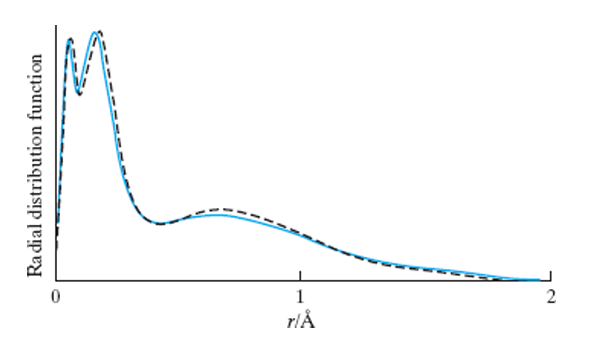
\includegraphics[width=0.65\textwidth]{Figures/11.1.png}
        \caption{
            \centering
            \parbox{0.6\linewidth}{
                \noindent
                \ce{Ar} 中径向分布函数与 $r$ 的函数关系。虚线是 Hartree–Fock 计算的结果。实线是电子衍射数据的结果。\\
                \small [Reprinted figure with permission from L.S. Bartell and L. O. Brockway, Physical Review Series II, Vol 90, 833, 1953. Copyright 1953 by the American Physical Society.]
            }
        }
        \label{fig:11.1}
    \end{figure}

    准确表示一个多电子原子轨道(AO)需要多个Slater型轨道的线性组合。对于粗略计算,使用简单的近似值来表示AO会更方便。我们可以使用具有有效核电荷的类氢轨道,但Slater提出了一种更简单的方法:用形式为(\ref{eq:11.14})的单一函数来近似AO,其中轨道指数$\zeta$取为
    \begin{equation}
        \zeta = \left(Z - s\right) / n
        \label{eq:11.15}
    \end{equation}
    其中$Z$为原子序数,$n$为轨道总量子数,$s$为屏蔽常数,可通过一组规则求得(见问题15.62)。Slater轨道用$r$的单次幂替换类氢轨道中$r$的多项式。因此,单个Slater轨道不具备正确的径向节点数,无法很好地表示轨道的内层部分。

    对多电子原子进行 Hartree–Fock SCF 计算(calculation)需要大量计算(computation)。在 20 世纪 30 年代,电子计算机尚未出现,Hartree 进行了多次 SCF 计算。幸运的是,Hartree 的父亲是一位退休工程师,他喜欢数字计算,并帮助了儿子。如今,计算机已经取代了 Hartree 的父亲。

\section{轨道和元素周期表}
\label{sec:11.2 Orbitals and the Periodic Table}














\section{电子相关}
\label{sec:11.3 Electron Correlation}

\section{角动量的叠加}
\label{sec:11.4 Addition of Angular Momenta}

\section{多电子原子的角动量}
\label{sec:11.5 Angular momentum in Many-Electron Atoms}

\section{自旋-轨道耦合}
\label{sec:11.6 Spin-Orbit Interaction}

\section{原子哈密顿算符}
\label{sec:11.7 The Atomic Hamiltonian}

\section{Condon-Slater规则}
\label{sec:11.8 The Condon-Slater Rules}

\section*{总结}

\section*{习题}
